\documentclass[11pt,a4paper]{article}
\usepackage[margin=1in]{geometry}
\usepackage{fontspec}
\usepackage{xeCJK}
\setCJKmainfont{Noto Sans CJK TC}
\usepackage{amsmath,amssymb}
\usepackage{graphicx}
\graphicspath{{results/}}
\usepackage{booktabs}
\usepackage{caption}
\captionsetup{font=small,labelfont=bf}
\usepackage[hidelinks]{hyperref}
\usepackage{enumitem}
\setlist{nosep,leftmargin=1.6em}
\usepackage{titlesec}
\titlespacing*{\section}{0pt}{1.2ex}{0.6ex}
\titlespacing*{\subsection}{0pt}{0.8ex}{0.4ex}

\newcommand{\Pit}{$P^{i}(t)$}

\title{\vspace{-1.2em}\textbf{The Value of Sharing Rebalancing Information on\\
YouBike Users' Waiting Cost:\\ A Data-Driven Time-Step Simulation}}
\author{Group 4 (CN-Team4)\\[0.45em]
\small
YU-CHIAN DUAN (B12902069) \quad PIN-HAO CHEN (B12902048) \quad BING-HAN LIN (B12902027)\\
YU-SIANG DENG (B12902004) \quad BO-HUNG SHEN (B12902075) \quad MING-LUNG TSAI (B12902078)\\[0.45em]
\normalsize Computer Networks Laboratory, National Taiwan University\\
\small\texttt{https://github.com/CN-Team4/final}}
\date{\today}

\begin{document}
\maketitle

\begin{abstract}
\noindent
Bike-sharing supply is highly uneven in space and time; during peak hours, popular stations frequently run out of bikes.
Operators rebalance the fleet with dispatch vehicles, but the location and timing of the dispatch fleet are known only to the
operator, not to users. This paper asks a question orthogonal to dispatch \emph{optimization}: under a fixed,
resource-constrained dispatch operation, does simply \emph{revealing} the current dispatch-vehicle locations to users reduce
their travel cost? We build a data-driven, time-step simulation of peak-hour shortage over a 76-station cluster around National
Taiwan University (NTU) and compare two scenarios---\emph{with} versus \emph{without} dispatch information---that share an
\emph{identical} dispatch supply (location and capacity); the only difference is whether users know where the dispatch bikes are.
The main metric is the difference in mean arrival time between the two scenarios, which isolates the value of the information
itself. All key quantities (hourly departure distribution, dispatch footprint, shortage rate, dock-fullness) are estimated from
$43.9$\,GB of real-time station-status data (Sept.\ 2025, weekdays) and monthly origin--destination statistics; the only purely
behavioral assumption is a detour-tolerance ratio $\tau$, for which we provide a sensitivity analysis. At NTU's empirically
measured shortage level ($\approx$32\%) and across a physically plausible dispatch capacity (50--200 bikes per peak window),
revealing dispatch locations lowers mean arrival time by \textbf{1.8--2.4 minutes (15--22\%)}; in the 10--20\% shortage range it
saves \textbf{2.4--3.2 minutes (22--31\%)}. The conclusion is robust to $\tau$. We further find that the operator's actual main
dispatch hub (MRT Gongguan, at the south-west edge) is sub-optimal for the campus shortage population, whose residual unmet
demand concentrates in the eastern dormitory/department area.

\smallskip
\noindent\textbf{Keywords:} bike sharing, information disclosure, rebalancing, agent-based simulation, network service design.
\end{abstract}

\section{Introduction}
\subsection{Problem and Motivation}
Public bike-sharing systems such as YouBike exhibit strong spatio-temporal demand imbalance, so that during peak hours certain
stations are emptied of bikes while others fill up. Operators counter this with \emph{dispatch vehicles} that move bikes between
stations. However, where and when these vehicles deposit bikes is internal operational information; a user who cannot find a bike
nearby has no way of knowing that a freshly replenished station exists a short walk away, and therefore resorts to guessing. We ask:
\begin{quote}\itshape
If the real-time location of the (already existing) dispatch bikes were disclosed to users---e.g., via an app layer---would it
shorten their time to destination?
\end{quote}
This is a network-service-design question about the effect of \emph{information disclosure} on system efficiency, deliberately
distinct from how to \emph{optimize} the dispatch policy.

\subsection{Our Angle}
Prior work mostly \emph{predicts} station occupancy or \emph{optimizes} the dispatch policy. Yet field reports indicate that real
dispatch is bottlenecked by limited vehicles, manpower, and turnaround speed, so a better policy does not automatically translate
into better service. We therefore hold the (limited) dispatch supply fixed and measure the marginal benefit of \emph{merely
revealing the existing dispatch information}. The study follows three principles:
\begin{enumerate}[label=(\arabic*)]
\item \textbf{Information is the only manipulated variable.} Both scenarios use the same dispatch locations, capacities, and counts;
they differ only in whether the user knows them. Biases in the data (existing rebalancing, censored demand) are common-mode and
cancel in the cost difference.
\item \textbf{No supply is added.} We quantify the marginal benefit of disclosing \emph{existing} dispatch locations, not of adding
vehicles.
\item \textbf{Replace assumptions with data.} Dispatch footprint, shortage rate, departure distribution, and dock-fullness are all
estimated from real data; the only behavioral assumption is the detour tolerance $\tau$, which we sweep.
\end{enumerate}

\subsection{Contributions}
(1) A data-driven peak-hour shortage simulation of the NTU YouBike cluster from two open datasets ($44$\,GB real-time dynamics +
monthly OD). (2) A quantification of the \emph{time value of dispatch-information disclosure}, and a two-dimensional
characterization (shortage level $\times$ dispatch quantity) of when it helps most. (3) An open-source, reproducible
implementation with interactive maps and an agent-movement animation.

\section{Related Work}
Prior studies cluster into prediction, dispatch optimization, and information services.
\begin{itemize}
\item \textbf{Occupancy prediction.} Yang~(2022)~\cite{yang2022} models future available-bike counts per station from history,
temporal features, and weather, exposed as a web service. \emph{Limitation:} answers ``how many bikes a station may have,'' not
rebalancing optimization.
\item \textbf{Dispatch optimization around NTU.} Chou~(2025)~\cite{chou2025} analyzes rental/return hotspots and ride times and
compares dispatch strategies (greedy, a survival-analysis SurvivalALG, and an offline near-optimal method). \emph{Limitation:}
the focus is ``how the operator should dispatch.''
\item \textbf{Zoning and routing optimization.} Ko~(2015)~\cite{ko2015} integrates depot location, zoning, vehicle count, and
routing cost and solves it with simulated annealing. \emph{Limitation:} suited to operator mid/long-term planning with
well-specified demand and routes.
\item \textbf{User-facing information services.} Chen et al.~(2022)~\cite{chen2022} propose app features (reservation, LED
displays, back-end statistics). \emph{Limitation:} argues users need better information but does not quantify how much time a
given piece of information saves.
\item \textbf{Operational constraints.} Su~(2023)~\cite{su2023} documents that the operator's dispatch vehicles, manpower,
throughput, and replenishment speed are tight, so even knowing which stations run dry does not guarantee timely replenishment.
\end{itemize}
\textbf{Gap.} Existing work optimizes policy or predicts occupancy; none quantifies the time benefit of disclosing \emph{existing}
dispatch information to users under a fixed, constrained dispatch operation---the question we address.

\section{Data}
\begin{table}[h]\centering\caption{Datasets.}\small
\begin{tabular}{p{3.0cm}p{2.0cm}p{6.0cm}}
\toprule
Source & Period & Use \\
\midrule
YouBike 2.0 real-time station dynamics ($\approx$43.9\,GB) & Sept.\ 2025, weekdays & Departure distribution \Pit; dispatch footprint; shortage rate; dock-fullness (from available bikes \texttt{sbi} and empty docks \texttt{bemp}) \\
Taipei YouBike OD statistics (data.taipei) & Dec.\ 2025, weekdays & Monthly OD demand $D_m^{ij}$; station graph \\
\bottomrule
\end{tabular}
\end{table}
The dynamics file is header-less; column meanings follow the official YouBike API schema and were verified against value
relationships (e.g., $\texttt{sbi}+\texttt{bemp}\approx\texttt{tot}$). We restrict to September 2025 weekdays (excluding the August
summer break and weekends) to align with the weekday OD data and the in-semester regime. Processing uses streaming reads on a
144-core machine ($\approx$60\,s per full pass); both datasets are fetched by \texttt{fetch\_data.sh}.

\section{System Model and Assumptions}
\subsection{Station Cluster (76 stations)}
Instead of an arbitrary radius, the cluster follows YouBike's official zoning:
\emph{NTU zone} $\cup$ stations named ``NTU'' (including the peripheral dormitory belt) $\cup$ the Gongguan exits (goal)
$-$ the downtown NTU-Hospital stations $=$ \textbf{76 stations}. Stations form a complete graph; distances are Manhattan; riding
speed is $5\times$ walking ($V_{\mathrm{walk}}=1.25$, $V_{\mathrm{bike}}=6.25$\,m/s).

\begin{figure}[h]\centering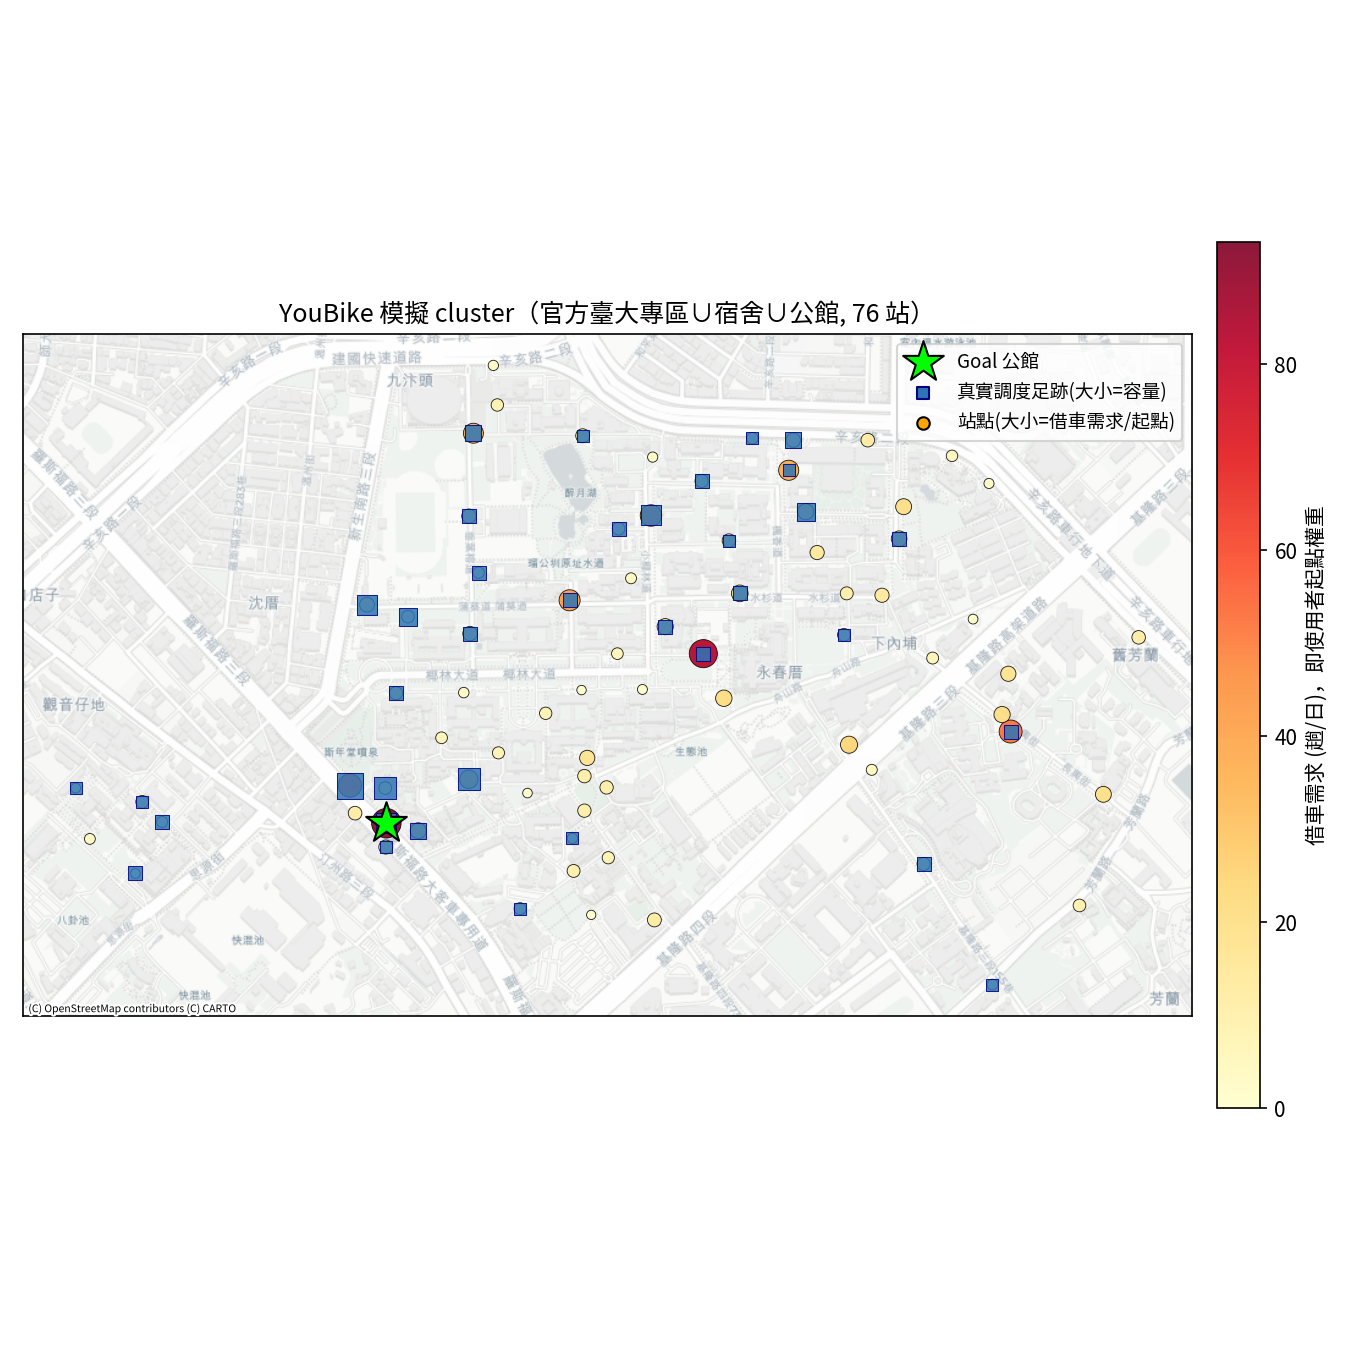
\includegraphics[width=0.86\textwidth]{map_cluster.png}
\caption{The 76-station NTU cluster. Blue squares mark the 37 data-detected dispatch stations (square size $\propto$ capacity);
red/orange/yellow dots show per-station borrow demand (larger dot $=$ higher origin weight). Cluster $=$ official NTU zone
$\cup$ ``NTU''-named stations (incl.\ the dormitory belt) $\cup$ Gongguan exits $-$ NTU-Hospital stations.}\label{fig:cluster}\end{figure}

\subsection{Dispatch Resource}
\textbf{Location/distribution} is detected from data: a single-step jump of $\ge 10$ in a station's available bikes is attributed
to a dispatch truck (ordinary returns add one at a time). Within the cluster, \textbf{37 stations} receive refills; their relative
shares come from the data. \textbf{Total quantity} is hard to measure: the detected total ($\approx$213 bikes/window) may be
inflated by return bursts, and the campus capacity is roughly $2$ trucks $\times 25$ plus on-site \emph{decompression} (bikes
stored beside a station and re-racked) and possibly multiple trips. We therefore \textbf{anchor the total at a physical
mid-estimate of 100 bikes per peak window} and treat it as an \emph{uncertain parameter}, sweeping a scale $s$ to
$25/50/100/200/400$; \textbf{50--200 is the plausible band}. Both scenarios use the identical footprint and capacity.

\subsection{Population and Behavior}
The population is the \emph{shortage group} (size $\alpha D_t$), spatially weighted by each station's measured peak
$\texttt{sbi}=0$ rate. Users are rational shortest-path agents and \emph{do not wait} (excluding a waiting branch isolates the
value of \emph{knowing the location}, not the side-effect of acting instead of waiting). Cars, ride-sharing, and reverse-direction
search are not modeled.

\section{Methodology}
\subsection{Demand Estimation}
\begin{equation}
D_d^{ij}=D_m^{ij}/N_d,\quad D_t^{ij}=D_d^{ij}\,P^{i}(t),\quad \text{shortage}=\alpha D_t^{ij} w_i,
\end{equation}
where $N_d$ is the weekday count, $P^i(t)$ the per-station hourly departure share, and $w_i$ a normalized shortage weight (so the
total shortage is $\alpha\sum D_t$ while its spatial pattern matches the measured shortage). The shortage ratio is
$\alpha/(1+\alpha)$; $\alpha$ is the swept variable.

\subsection{Empirical Estimation}
\textbf{\Pit:} between consecutive status changes, a drop in \texttt{sbi} counts as a borrow; borrows are aggregated by hour and
normalized per station (1{,}651 stations). The simulation uses each origin's own \Pit\ (the cluster curve is shown only for
illustration); the NTU curve is multi-peak ($\approx$09{:}00, 13{:}00, 17{:}00) with peak window 17{:}00--19{:}00.
\textbf{Shortage rate:} the peak $\texttt{sbi}=0$ time fraction, demand-weighted $f\approx 32\%$, i.e.\ $\alpha\approx0.48$.
\textbf{Dock-fullness:} peak fraction with $\texttt{bemp}\le 2$ ($\approx$80--90\% at the Gongguan exits), used for return cost.

\subsection{User Decision and Cost (no waiting)}
\textbf{Without information:} walk to the single nearest station; if it is a dispatch station with capacity, ride to the
destination; otherwise walk on. \textbf{With information:} walk to the nearest dispatch station within tolerance
$\tau\cdot\mathrm{dist}(i,j)$ that still has capacity and ride; if none, walk. Let $nv$ be the station nearest to destination $j$
and $f_{\mathrm{full},j}$ its measured fullness; a rider's expected return detour is
\begin{equation}
\mathrm{ret}_j=f_{\mathrm{full},j}\big(\mathrm{dist}(j,nv)/V_{\mathrm{bike}}+\mathrm{dist}(nv,j)/V_{\mathrm{walk}}\big).
\end{equation}
The resulting cost has three cases. (i) \emph{Reach a bike at station $x$ and ride} (with-info success at $x{=}g$, or
without-info success when the nearest station $m$ is a dispatch station): $\mathrm{dist}(i,x)/V_{\mathrm{walk}}+
\mathrm{dist}(x,j)/V_{\mathrm{bike}}+\mathrm{ret}_j$. (ii) \emph{With-info give-up} (no reachable dispatch): walk straight to
the destination, $\mathrm{dist}(i,j)/V_{\mathrm{walk}}$. (iii) \emph{Without-info miss} (the nearest station $m$ is not a
dispatch station): walk via $m$, $\mathrm{dist}(i,m)/V_{\mathrm{walk}}+\mathrm{dist}(m,j)/V_{\mathrm{walk}}$.

\subsection{Simulation}
A time-step simulation allocates each dispatch station's capacity first-come (by arrival order). Each (scenario, parameter)
combination runs 30 Monte-Carlo repetitions (Poisson shortage counts); we report means with 95\% confidence intervals. Both
scenarios use the same agents and capacities.

\section{Experimental Setup}
\textbf{Exp.\ 1:} fix the real footprint ($s{=}1$, $\tau{=}0.5$) and sweep $\alpha$. \textbf{2-D sweep:} $\alpha\times s$ (shortage
$\times$ dispatch quantity). \textbf{$\tau$ sensitivity:} sweep $\tau\times\alpha$. \textbf{Appendix:} concentrate the total
capacity at a single station and sweep all 76 to find the best location. \textbf{Baseline:} without information.
Environment: Python~3.14, polars, NumPy, Matplotlib, Folium (Leaflet), contextily.

\section{Results}
\begin{figure}[h]\centering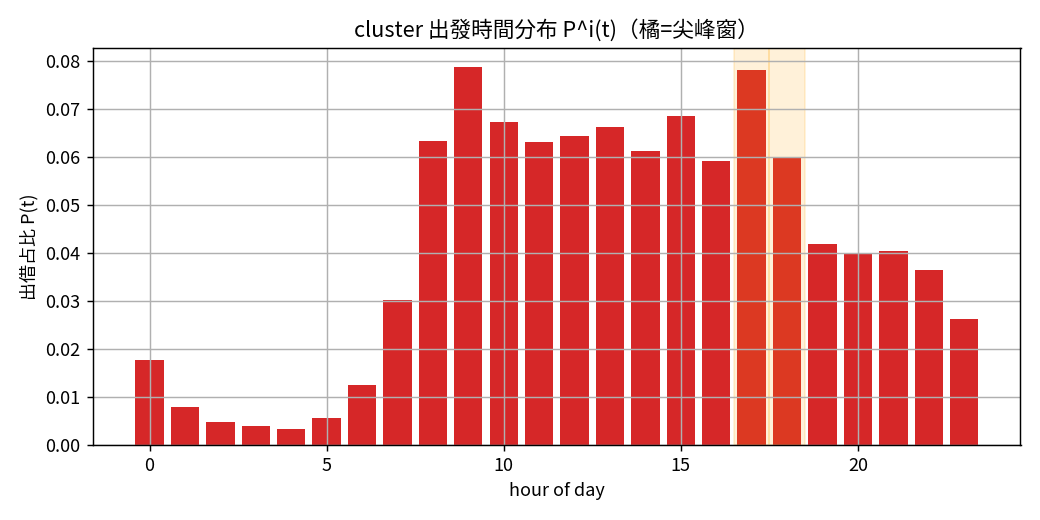
\includegraphics[width=0.92\textwidth]{pit_cluster.png}
\caption{Cluster-aggregate departure distribution \Pit\ (campus multi-peak; orange = peak window). The simulation uses each
station's own \Pit.}\label{fig:pit}\end{figure}

At the operating point ($\alpha\approx0.48$, capacity $=100$), the share of shortage users obtaining a bike rises from
$\approx$6\% (without) to $\approx$15\% (with) information ($\approx 2.5\times$).

\begin{figure}[h]\centering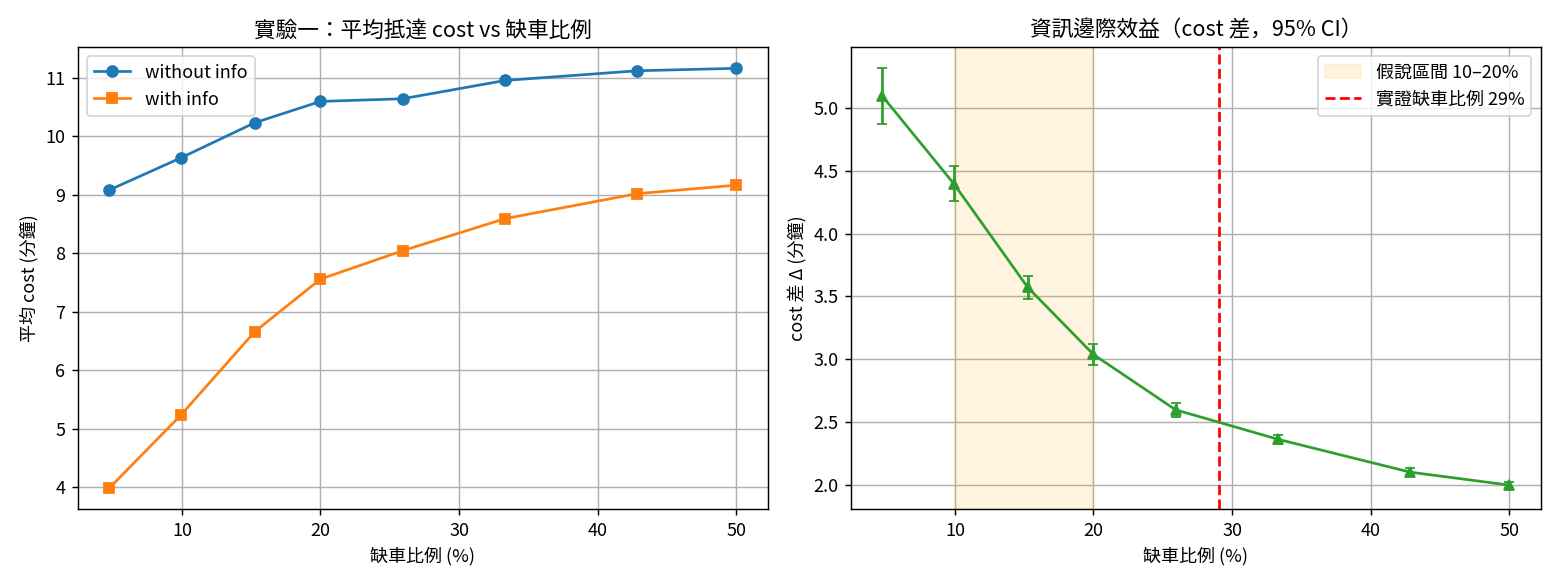
\includegraphics[width=\textwidth]{exp1_alpha.png}
\caption{Exp.\ 1. Left: mean arrival cost per scenario. Right: cost difference $\Delta$ (95\% CI); orange band = 10--20\%
hypothesis range, red dashed line = empirical $\approx$32\% shortage. Dispatch capacity $=100$ bikes/window.}\label{fig:exp1}\end{figure}

\begin{table}[h]\centering\caption{Exp.\ 1 (capacity $=100$ bikes/window).}\small
\begin{tabular}{rrrrr}
\toprule
Shortage & Without & With & $\Delta$ (saved) & Relative \\
\midrule
4.8\%  & 9.8 min & 5.4 min & \textbf{4.4 min} & 45\% \\
9.9\%  & 10.4 & 7.1 & \textbf{3.2} & 31\% \\
15.3\% & 10.8 & 8.1 & \textbf{2.7} & 25\% \\
20.0\% & 11.0 & 8.6 & \textbf{2.4} & 22\% \\
25.9\% & 11.1 & 8.9 & 2.2 & 19\% \\
33.3\% & 11.3 & 9.3 & 2.0 & 18\% \\
50.0\% & 11.5 & 9.7 & 1.8 & 15\% \\
\bottomrule
\end{tabular}
\end{table}

Mean cost without information is $\approx$10--11\,min, flat in $\alpha$ (random search is insensitive to shortage); with
information it rises as the dispatch capacity saturates. The hypothesis holds: at 10--20\% shortage information saves
\textbf{2.4--3.2\,min (22--31\%)}; at the empirical $\approx$32\% it still saves $\approx$2.0\,min (18\%).

\begin{figure}[h]\centering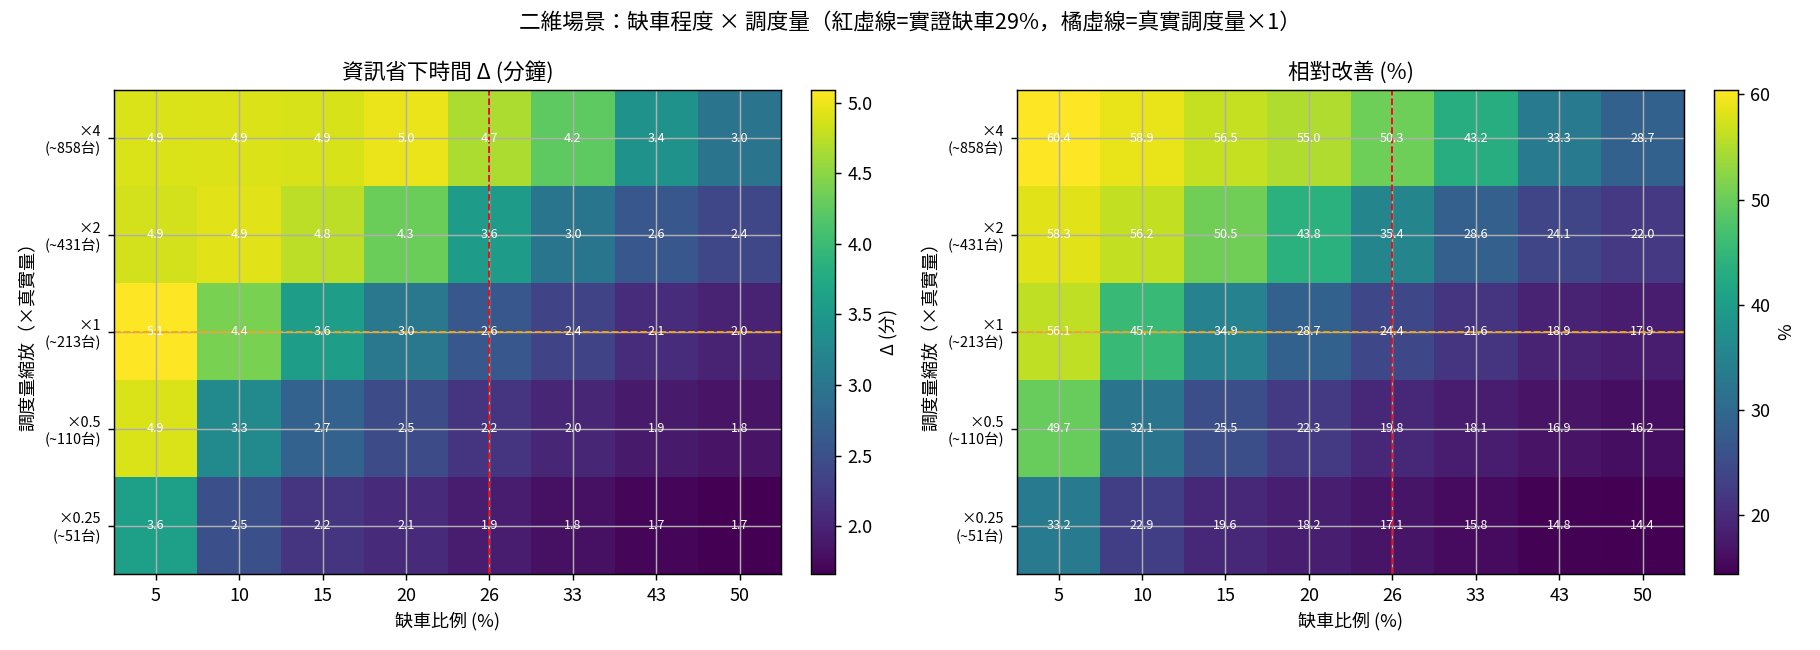
\includegraphics[width=\textwidth]{heatmap.png}
\caption{$\Delta$ (min) and relative improvement (\%) over shortage $\times$ dispatch quantity. Red line = empirical shortage,
orange line = mid-estimate 100 bikes, white box = plausible band 50--200.}\label{fig:heat}\end{figure}

Information is most valuable when shortage is low and dispatch ample (upper-left). Within the plausible band at the empirical
shortage, the improvement is \textbf{15--22\% ($\Delta\approx$1.8--2.4\,min)}; raising dispatch from $\approx$50 to $\approx$400
bikes lifts it from $\approx$15\% to $\approx$29\%.

\begin{figure}[h]\centering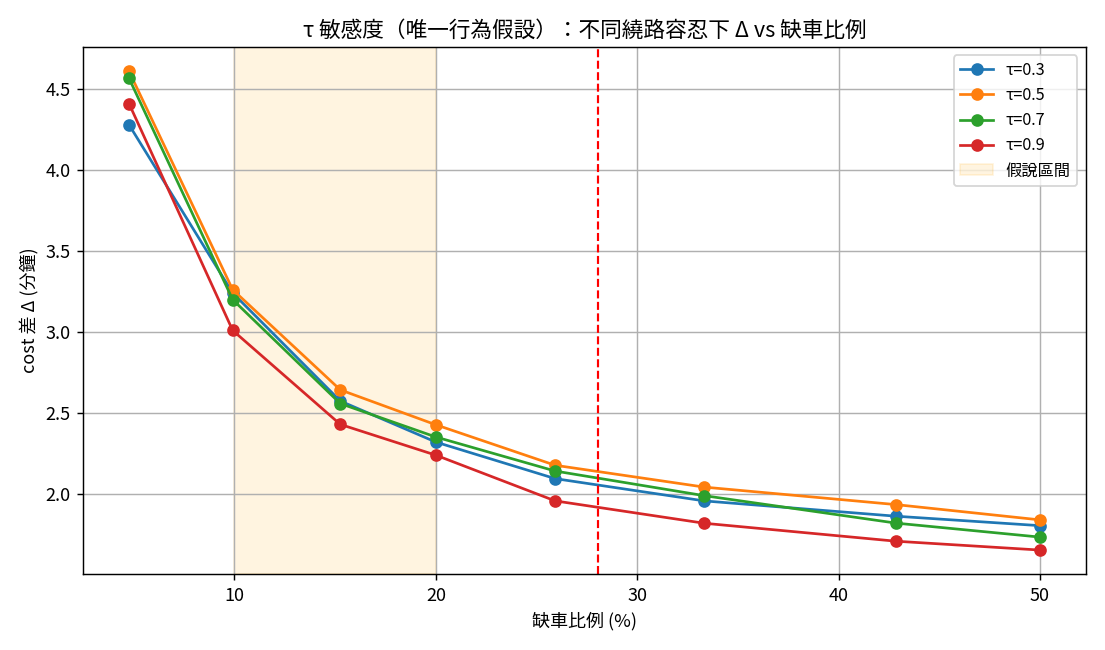
\includegraphics[width=0.92\textwidth]{tau_sensitivity.png}
\caption{$\Delta$ vs shortage for $\tau\in\{0.3,0.5,0.7,0.9\}$.}\label{fig:tau}\end{figure}

Across the full $\tau$ range the curves differ by less than $0.5$\,min with no consistent direction: the dense real footprint
makes the tolerance rarely bind, so the conclusion does not depend on $\tau$.

\begin{figure}[h]\centering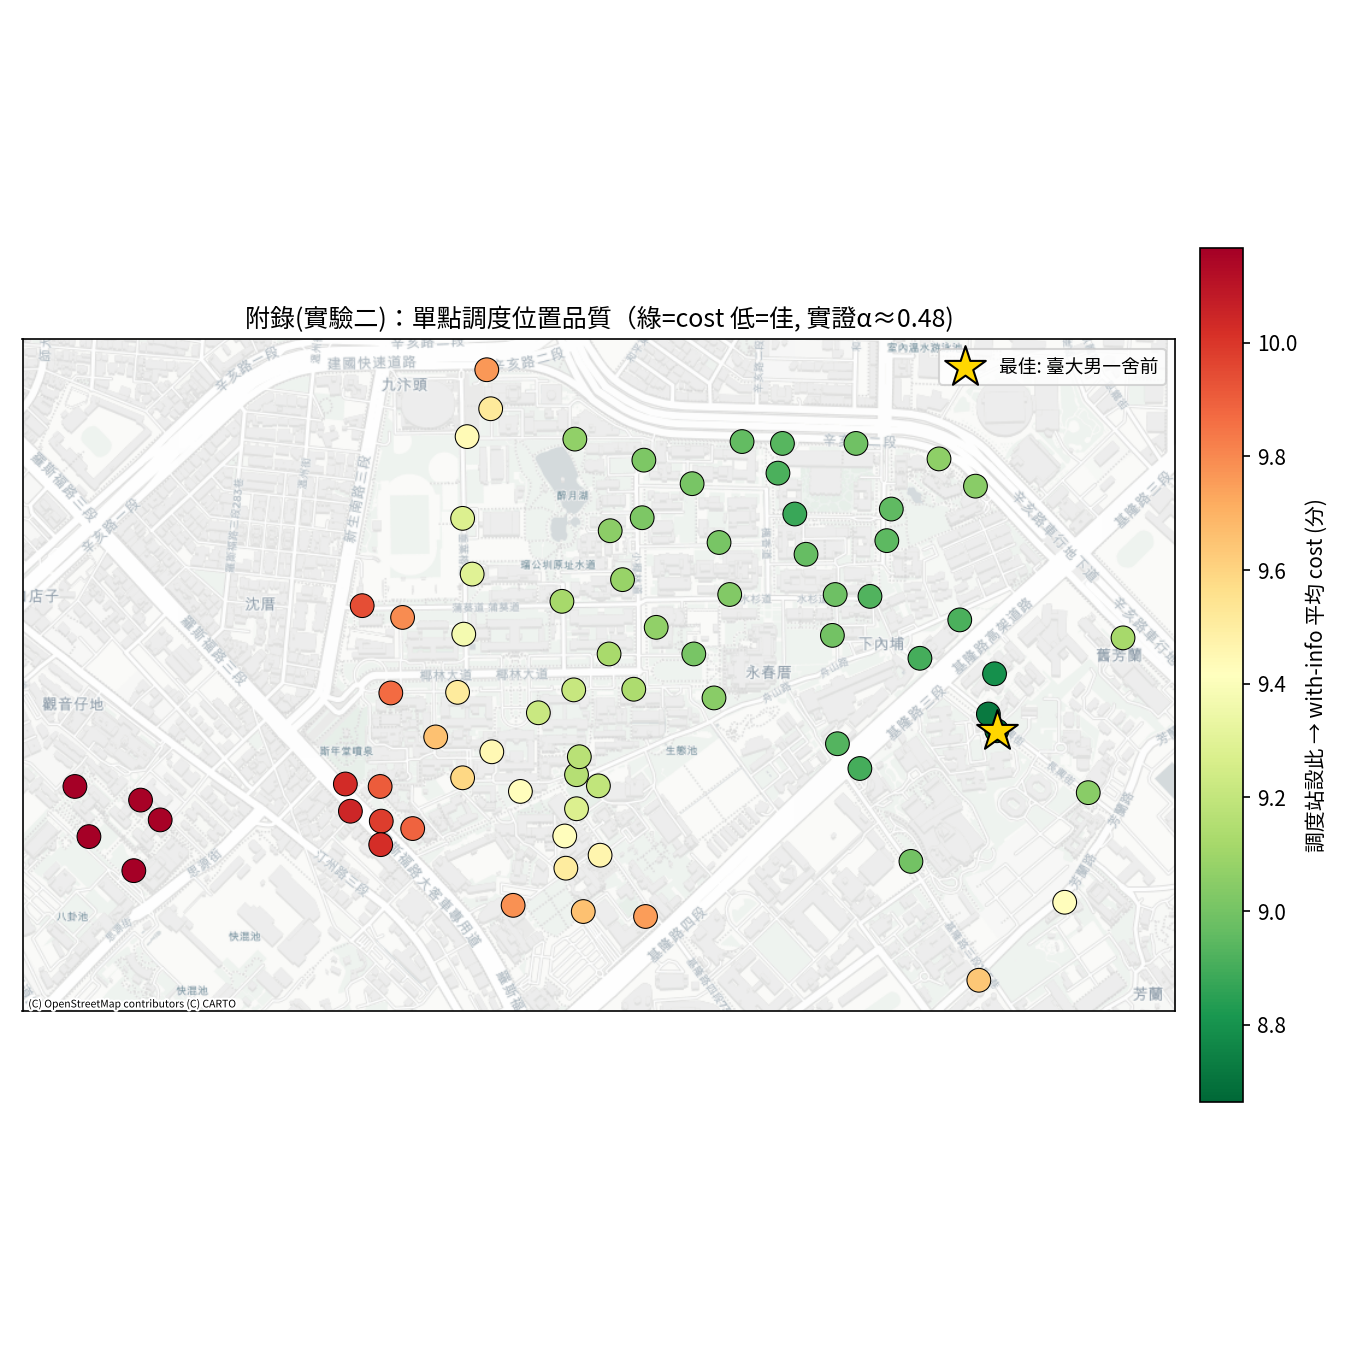
\includegraphics[width=0.78\textwidth]{map_exp2.png}
\caption{With-info mean cost when the total capacity is concentrated at each candidate station (green = better).}\label{fig:exp2}\end{figure}

When concentrated at a single station, the best locations lie in the \textbf{eastern dormitory/department area} (around Men's
Dormitory~1 and Mingda Hall), near the most shortage-prone interior stations (second EE building 62\%, Forestry building 57\%).
The current main hub, MRT Gongguan, sits at the south-west edge and is sub-optimal for the campus shortage population. An
agent-movement animation (\texttt{results/anim.html}) shows the two scenarios side by side on a shared clock.

\section{Discussion}
\textbf{Why information helps:} the dominant cost is walking far after failing to find a bike; information turns ``gamble at the
nearest station'' into ``head to a dispatch station that certainly has a bike within an acceptable detour,'' replacing walking
with riding. \textbf{Complementarity:} information needs sufficient dispatch to point users toward; under extreme shortage the
capacity saturates and the marginal benefit falls. \textbf{Relation to prior work:} whereas others optimize the policy---limited
in practice by manpower and vehicles~\cite{su2023}---we show that under the \emph{same} constrained supply, disclosing existing
locations already yields a sizeable, near-zero-cost saving (an app layer). \textbf{Policy:} for further gains, placing dispatch
resources in the eastern campus area is more efficient than reinforcing the peripheral Gongguan hub.

\section{Limitations}
Dispatch quantity is the largest uncertainty (proxy detection, no official records, possible return-burst inflation; hence
anchored at a physical estimate and swept 50--200). Temporal mismatch: dynamics from Sept.\ 2025 vs.\ OD from Dec.\ 2025.
Without information, users try only the single nearest station. Shortage is approximated by the $\texttt{sbi}=0$ time fraction.
Return cost is an expected-value approximation. Waiting, cars, and ride-sharing are not modeled.

\section{Conclusion}
Disclosing the locations of the existing dispatch bikes measurably shortens peak-hour arrival time on the NTU campus: at the
empirical $\approx$32\% shortage across a plausible dispatch capacity (50--200 bikes/window) it saves $\approx$1.8--2.4\,min
(15--22\%), and 2.4--3.2\,min (22--31\%) in the 10--20\% range. The result is robust to the only behavioral assumption $\tau$.
Information and supply are complementary; given that real dispatch is resource-constrained, information disclosure is a low-cost
lever that complements rather than replaces dispatch optimization. The study is data-driven and openly reproducible.

\section*{Author Contributions}
All six members contributed equally (1/6 each).
\begin{table}[h]\centering\small
\begin{tabular}{p{4.4cm}p{2.2cm}p{7.6cm}}
\toprule
Member & Student ID & Role \\
\midrule
段宇謙 (YU-CHIAN DUAN) & B12902069 & Data integration and empirical statistics (44\,GB real-time dynamics) \\
陳品豪 (PIN-HAO CHEN) & B12902048 & Algorithm and simulation implementation \\
林秉翰 (BING-HAN LIN) & B12902027 & Project proposal, slides, oral presentation \\
鄧育翔 (YU-SIANG DENG) & B12902004 & Slides, oral presentation \\
沈柏宏 (BO-HUNG SHEN) & B12902075 & Report writing \\
蔡明龍 (MING-LUNG TSAI) & B12902078 & Report writing \\
\bottomrule
\end{tabular}
\end{table}

{\small
\bibliographystyle{unsrt}
\bibliography{references}}

\end{document}
